\section{Spin Polarisation}\label{spin_polarisation}
% \cite{2008}\cite{Weil2006}\cite{Goldfarb2018-he}\cite{Richert2017}
Spin polarisation in the context of EPR is the unequal population of possible spin states. Ordinarily the population of each spin sub-level is governed by \index{Boltzman statistics}{Boltzman statistics}, thus above cryogenic temperatures, there is no preferential spin sub-level.

For a two-level system at temperature $T$, statistical mechanics tells us that the probability to
be in state $\ket{i}$ is given by 
\begin{equation}
    p(\ket{i}) = \frac{e^{E_i / k_B T}}{e^{E_0 / k_B T} + e^{E_0 / k_B T}}.
    \label{eq:boltzman_prob}
\end{equation}

If we then consider a two level system $S= 1/2$ under the influence of the Zeeman effect (\ref{zeeman}), the difference in energy is $\Delta E = \gamma B$. Using \eqref{eq:boltzman_prob} we find 
\begin{equation}
    p(\ket{+}) = \frac{e^{ \gamma B / 2 k_B T}}{e^{\gamma B / 2 k_B T} + e^{- \gamma B /2 k_B T}} = \frac{1}{1 + e^{-\gamma B/2 k_B T}}.
    \label{eq:boltzman_specific_state}
\end{equation}

It is easy to see from \eqref{eq:boltzman_specific_state} for room temperature, the probability is around $50\%$. 

We define the polarisation as the normalised difference between the probability of population of two states as 
\begin{equation}
    P = \frac{p(\ket{+}) - p(\ket{-})}{p(\ket{+}) + p(\ket{-})}.
    \label{eq:spin_polarisation}
\end{equation}

Substituting \eqref{eq:boltzman_prob} for our two level system, we see that even in strong magnetic fields the spin states remain unpolarised even when temperature is as low as a few K. However, when we approach $\mathcal{O}(10^{-3})$ K we see polarisation approach $100\%$ with as little as $0.1$ T applied \cite{Bonato}.  

% For example the differing population of triplet sublevels under the influence of photoexcitation. 
% Microwave radiation is only absorbed or emitted in a spin polarised system; so spin polarisation is essential for EPR. 

Despite this, it is possible to induce a spin polarisation above cryogenic temperatures and one technique to achieve this is optical polarisation.

% BOLTZMAN STATISTICS

\subsection{Optical Polarisation}
% We find that simultaneous optical reionization and qubit manipulation can be carried out at room temperature with photoexcitation at the typical excitation wavelength used for readout of the divacancy qubits in 4H SiC


For the systems described in this work, optical polarisation is achieved via a Stokes excitation, moving the electron from the ground state to an excited state \cite{PhysRevB.105.165108}. This will naturally decay either via a spin preserving transition (which will emit a photon) or a non-spin preserving transition which in general do not emit a photon in the measured frequency range and are referred to as dark states.

These dark decay routes will preferentially reduce the electron to the $m_s = 0$ ground state and on average take a lot longer than the spin preserving transitions.

\begin{figure}
	\begin{center}
		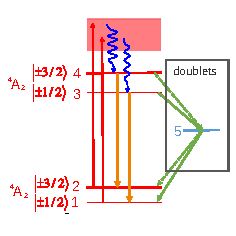
\includegraphics[width=0.5\textwidth]{figures/actual-stokes.pdf}
% The red (dark brown) arrows represent optical excitation from the ground state (labels 1 and 2) toward the excited states
% (labels 3 and 4) and the yellow arrows represent the associated spin-preserved radiative decay. The green arrows represent intersystem crossing (ISC)
% routes where dotted arrows mean weaker transitions than those represented by straight arrows. Blue wavy arrows show the phonon-related decay and
% excitation routes that are temperature dependent
		\caption{Energy level diagram for a $S=3/2$ system showing Stokes excitation (red), spin-preseving radiative decay (orange), dark decay routes (green) where the solid arrow is a stronger transition and phonon related decay (blue). Adapted from Wang et al.}\label{fig:big_stokes}
	\end{center}
    % \todo[inline, color=ediblue]{Write caption}
\end{figure}


Polarisation is achieved in the steady state when the defect is illuminated for several excitation/decay cycles. A simple description with reference to figure \ref{fig:big_stokes} is:
\begin{enumerate}
    \item The laser is incident on the defect (red arrows) and fast, spin preserving, radiative decays occur 
        taking $m_s = \pm1/2$ excited states to $m_s = \pm1/2$ ground states (and similar for $m_s = \pm3/2$). 
    \item A proportion of the electrons decay via the non-spin-preserving dark routes (green arrows), 
        for which the solid arrow occurs most often. 
    \item Since the solid green arrow is preferred, over several cycles, most of 
        the electrons end up decaying to the $m_s = \pm 1/2$ ground state, 
        where they will be "stuck" in the much faster, spin preserving cycle. Any dark decay, will return the electron to the $m_s = \pm 1/2$
    \item The result is a system within which most of the electrons are in the $m_S = \pm 1/2$ state. 
\end{enumerate}

The process above is a simplification of the actual process but qualitatively describes the process. Optical polarisaion has been demonstrated in SiC and shown to achieve $99 \pm 1$\% polarisation which is equivalent to reducing the temperature to $5 \mu$K
% The 99 +/- 1% degree of polarization at room temperature corresponds to an effective nuclear temperature of 5 microKelvin. 
\cite{polarisation}
.

\subsection{Rabi Oscillations}
From a polarised state, the unequal population of the spin sub-levels is brought back to equilibrium either by the thermodynamic effect (a return to the Boltzman distribution) or by an induced magnetic resonance transition, known as a Rabi oscillation. The Rabi oscillation is what is exploited in EPR and produces a detectable change in photoluminescence in the ODMR spectra.

A driving magnetic field is applied to the system to induce a transition between the $m_s = \pm 1/2$ and the $m_s = \pm 3/2$ sub-levels in the ground state. This will disrupt the steady state of the system achieved by point $4$ in the list above and force a change in photoluminescence which may be detected. 

